\documentclass[NET,english,aspectratio=169,notitleframe]{tumbeamer}
%settings
\usepackage[utf8]{inputenc}
\usepackage{pgfplotstable}
\usepackage{marvosym}
\usepackage{filecontents}
\usepackage{packages}
\usepackage{beamermods}

\usepackage[backend=bibtex, style=ieee]{biblatex}

\usepackage{csquotes}

\usetikzlibrary{calc}
\usetikzlibrary{arrows.meta}


% For lecture mode (use package option 'lecture'):
%\lecture[GRNVS]{Grundlagen Rechnernetze und Verteilte Systeme}
%\module{IN0010}
%\semester{SoSe\,2016}
%\assistants{Johannes Naab, Stephan Günther, Maurice Leclaire}

\usepackage{pgfplots}
\pgfplotsset{compat=newest}
\usepackage{tumcolor}
\usepackage{tumcolors}
\usepackage{textpos}


\usepackage{pgfpages}
\usepackage{ifthen}
% ============================================================================
% jobname solution
% ============================================================================
\newif\ifsolution%
\ifthenelse{\equal{\detokenize{notes}}{\jobname}}{%
\setbeameroption{show notes on second screen=bottom}
\setbeamercolor{note page}{bg=white, fg=black}
\setbeamercolor{note title}{bg=white!95!black, fg=black}
}{
}

%\xdefinecolor{orange}{cmyk}{0,0.65,0.95,0} 
%\xdefinecolor{dblue}{cmyk}{1,0.54,0.04,0.19}
%\xdefinecolor{blue}{cmyk}{1,0.43,0,0}  
%\xdefinecolor{lblue}{cmyk}{0.65,0.19,0.01,0.04}
%\xdefinecolor{green} {cmyk}{0.35,0,1,0.2} 
%xdefinecolor{yellow}{rgb}{1.00,0.71,0.00} 
%\colorlet{lgtorange}{orange!20} 
%\colorlet{lgtdblue}{dblue!20} 
%\colorlet{lgtblue}{blue!20} 
%\colorlet{lgtlblue}{lblue!20} 
%colorlet{lgtgreen}{green!20} 
%\colorlet{lgtyellow}{yellow!20}

\newcommand\Wider[2][3em]{%
\makebox[\linewidth][c]{%
  \begin{minipage}{\dimexpr\textwidth+#1\relax}
  \raggedright#2
  \end{minipage}%
  }%
}
\usepackage{cancel}
\usepackage{minted}


\addbibresource{lit.bib}


% For beamer mode (default):
 % jeder von dem wir hier irgendwas nehmen, alphabetisch sortiert
\author[Paul Emmerich, Simon Ellmann, Sebastian Voit]{\textbf{Paul Emmerich}, \textbf{Simon Ellmann}, \textbf{Sebastian Voit},\\ Fabian Bonk, Alex Egger, Alexander Frank, Thomas Günzel,\\ Stefan Huber,  Maximilian Pudelko, Maximilian Stadlmeier}
\title{Safe and Secure Drivers in High-Level Languages}
\date{December 29, 2018}

\makeatletter
\let\@@magyar@captionfix\relax
\makeatother

\begin{document}

\setbeamertemplate{footline}{}
  \begin{frame}[c,noframenumbering]
%    \begin{tikzpicture}[overlay,remember picture]
%      \node[opacity=0.5,anchor=south east] at ($(current page.south east)+(-1,-1)$) {%
%    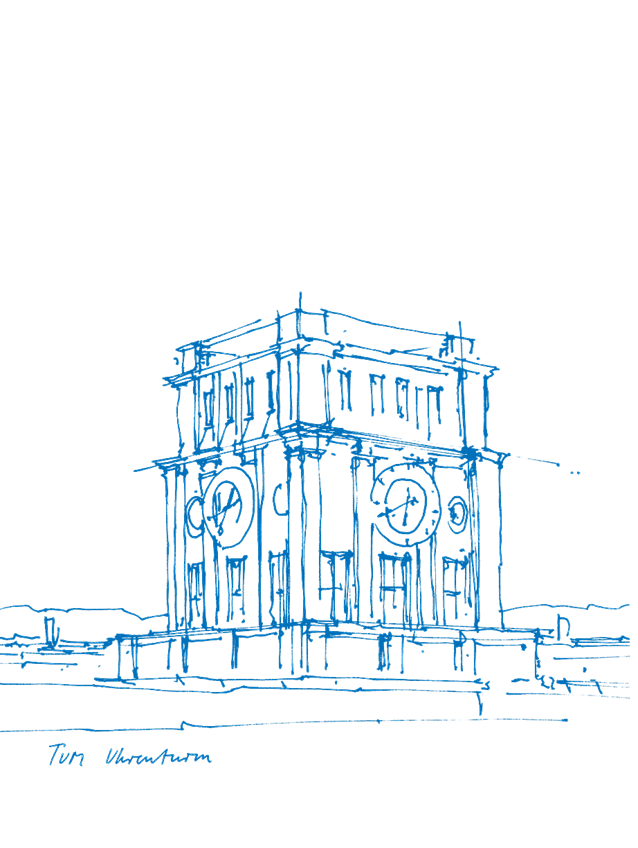
\includegraphics[width=.4\textwidth]{pics/TUM_Uhrenturm.png}};
%  \end{tikzpicture}
  \centering%
  \Large%
  \strut\textcolor{TUMBlue}{\inserttitle}%
  \\[4ex]%
  \normalsize%
  \strut\insertauthor%
  \\[2ex]%
  \footnotesize%
  \insertdate%
  \\[4ex]%
  \ifdefined\departmentname%
    \ifdefined\chairname%
      \chairname\\%
    \fi%
    \departmentname\\%
  \fi%
  \TUMname\\%
\end{frame}

  \begin{frame}[c,noframenumbering]
%    \begin{tikzpicture}[overlay,remember picture]
%      \node[opacity=0.5,anchor=south east] at ($(current page.south east)+(-1,-1)$) {%
%    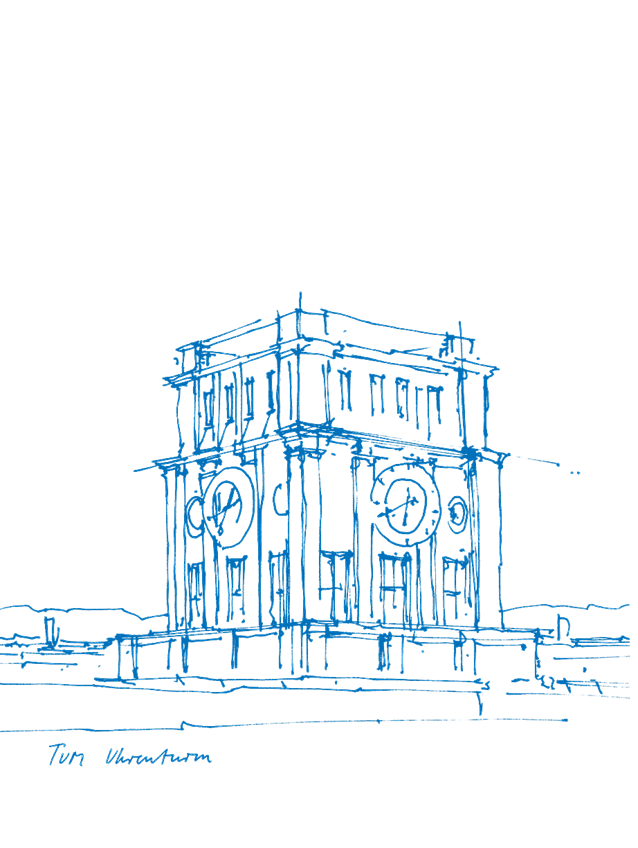
\includegraphics[width=.4\textwidth]{pics/TUM_Uhrenturm.png}};
%  \end{tikzpicture}
  \centering%
  \Large%
  \strut\textcolor{TUMBlue}{\inserttitle}%
  \\[4ex]%
  \normalsize%
  \strut{}\bfseries Paul Emmerich$^1$, Simon Ellmann$^2$, Sebastian Voit$^3$,\\ Fabian Bonk$^4$, Alex Egger$^5$, Alexander Frank$^6$, Thomas Günzel$^7$,\\ Stefan Huber$^8$, Maximilian Pudelko$^9$, Maximilian Stadlmeier$^{10}$ \normalfont %
  \\[2ex]%
  \footnotesize%
  $^1$C, thesis advisor\hspace{1em}
  $^2$Rust\hspace{1em}
  $^3$Go\hspace{1em}
  $^4$OCaml\hspace{1em}
  $^5$Haskell\hspace{1em}\\
  $^6$Latency measurements\hspace{1em}
  $^7$Swift\hspace{1em}
  $^8$IOMMU\hspace{1em}
  $^9$VirtIO driver\hspace{1em}
  $^{10}$C\#\hspace{1em}
  \\[4ex]%
    \ifdefined\departmentname%
    \ifdefined\chairname%
      \chairname\\%
    \fi%
    \departmentname\\%
  \fi%
  \TUMname\\%
\end{frame}
\setbeamertemplate{footline}[tumfootline]

\begin{frame}{About us}
\begin{columns}
\begin{column}{0.8\textwidth}
\emph{Paul}
\begin{itemize}
\item PhD student at Technical University of Munich
\item Researching performance of packet processing systems
\end{itemize}
\vfill
\emph{Simon}
\begin{itemize}
\item Rust driver as bachelor's thesis, now HiWi/research assistant
\end{itemize}
\emph{Sebastian}
\begin{itemize}
\item Go driver as bachelor's thesis
\end{itemize}
\emph{Everyone else}
\begin{itemize}
\item Did a thesis with Paul as advisor
\end{itemize}
\end{column}
\begin{column}{0.15\textwidth}
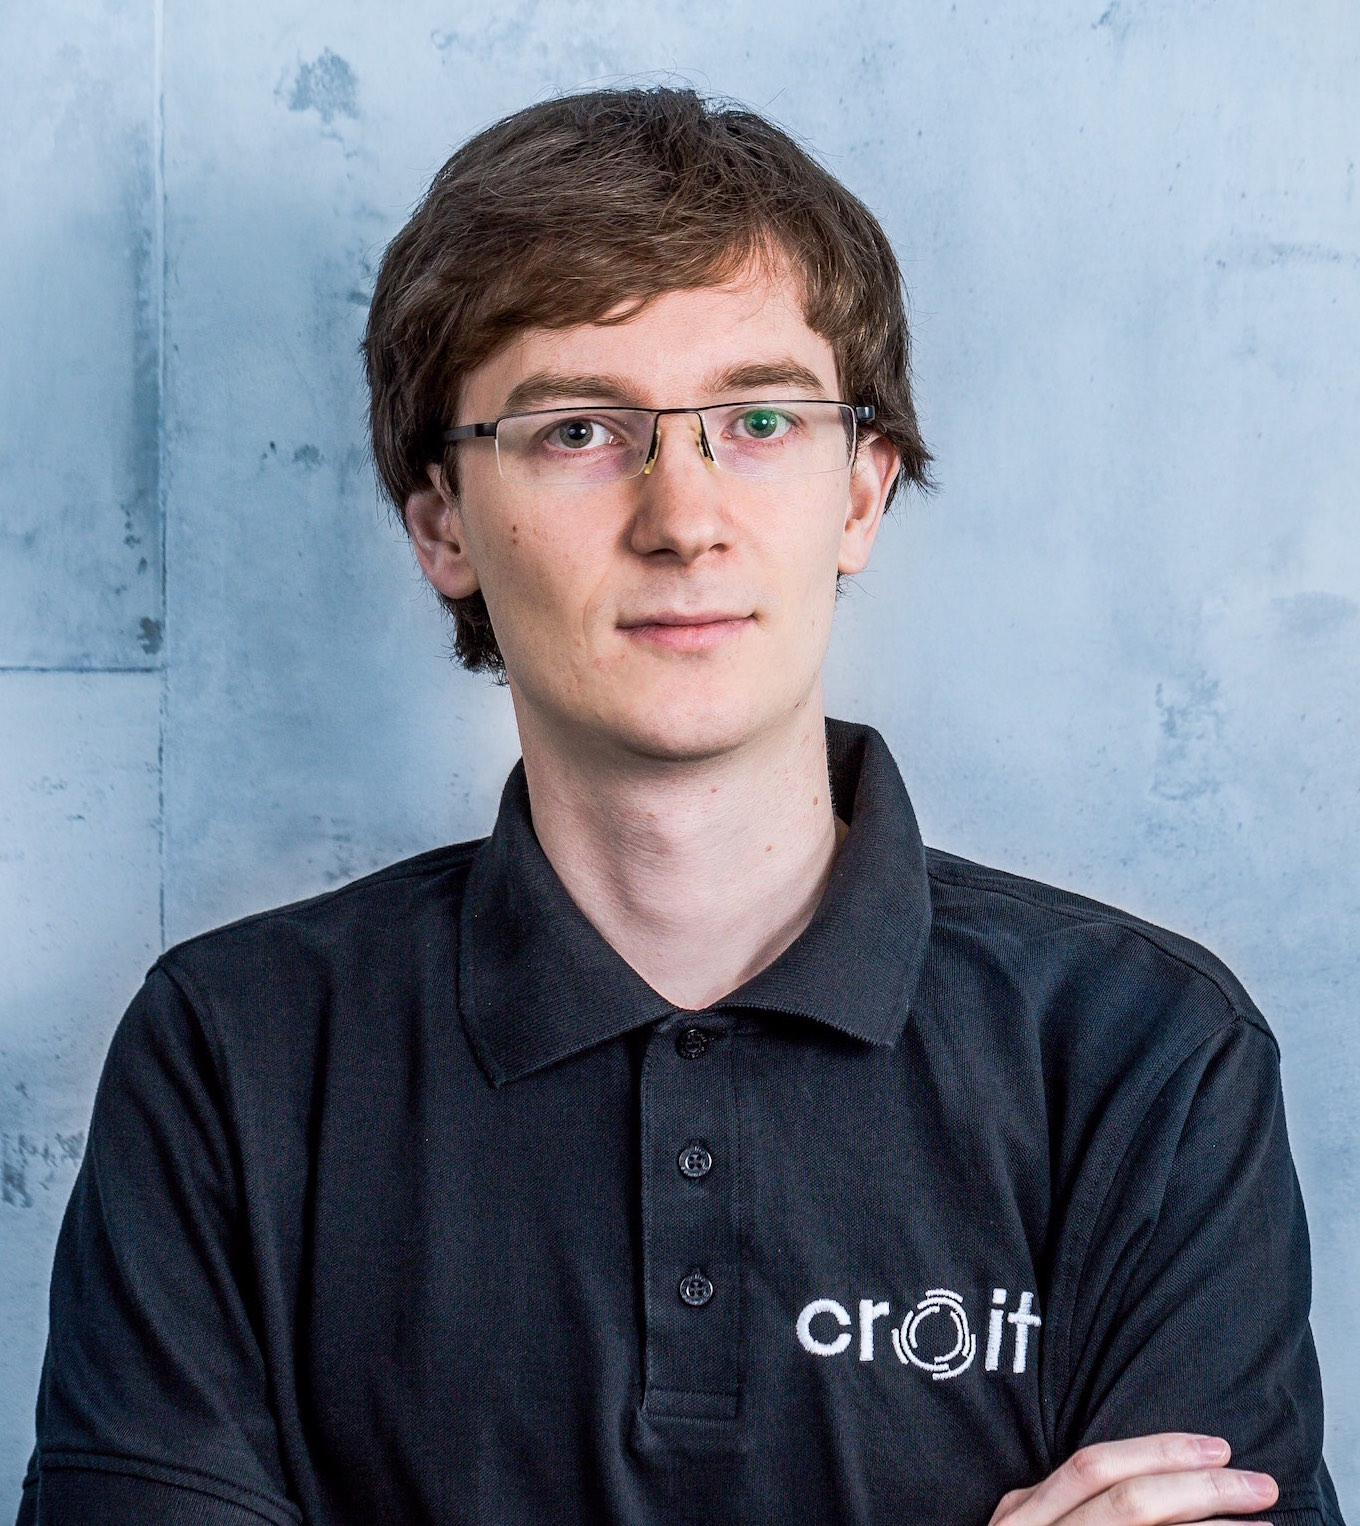
\includegraphics[width=0.8\textwidth]{pics/paul.jpg}\\
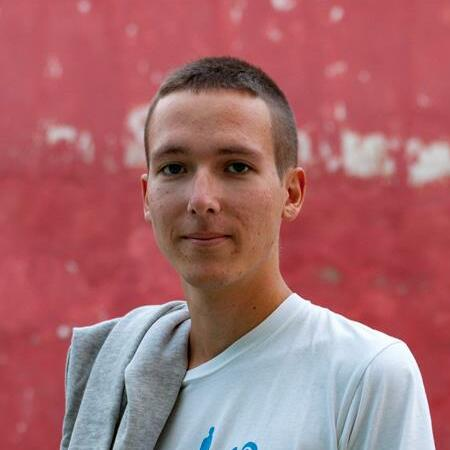
\includegraphics[width=0.8\textwidth]{pics/simon.jpg}\\
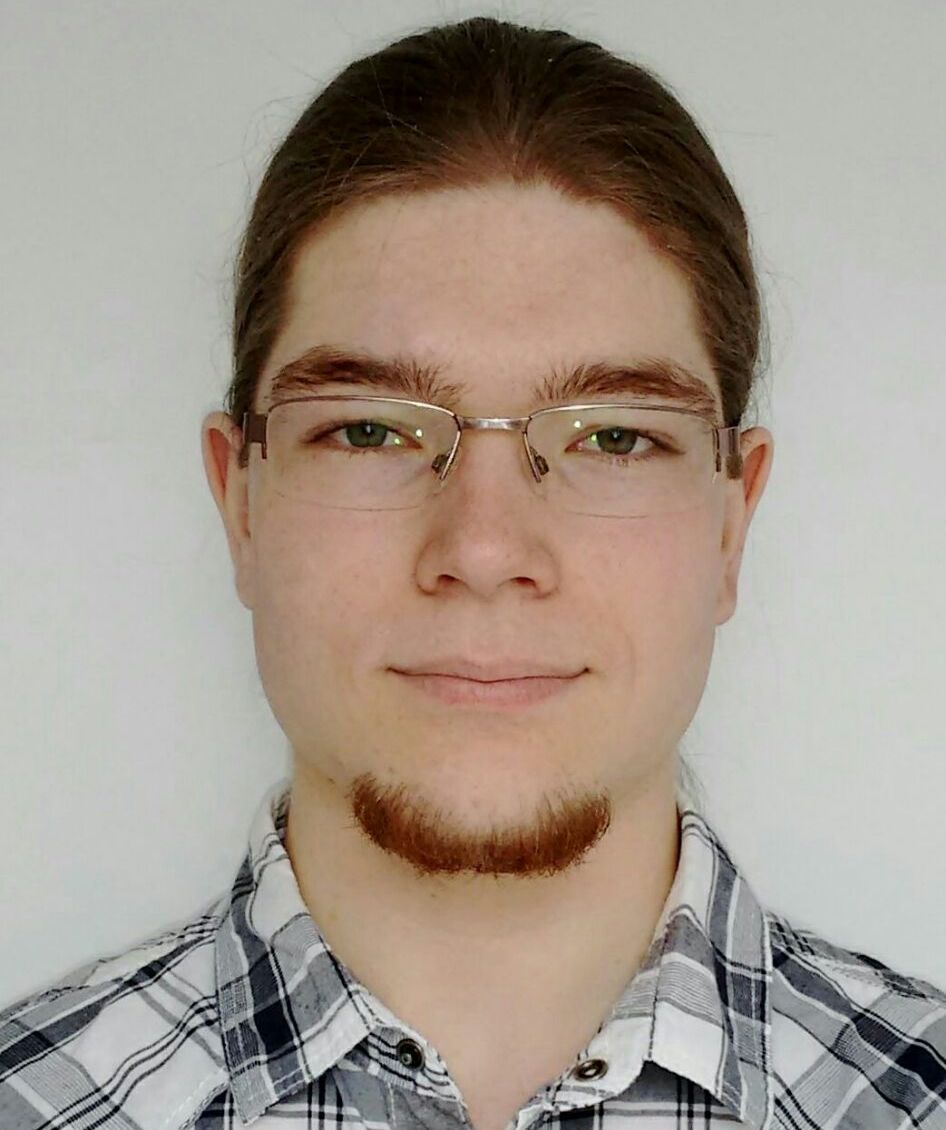
\includegraphics[width=0.8\textwidth]{pics/sebastian.jpg}
%\end{tikzpicture}
\end{column}
\end{columns}
\end{frame}


\begin{frame}{Network drivers}
\centering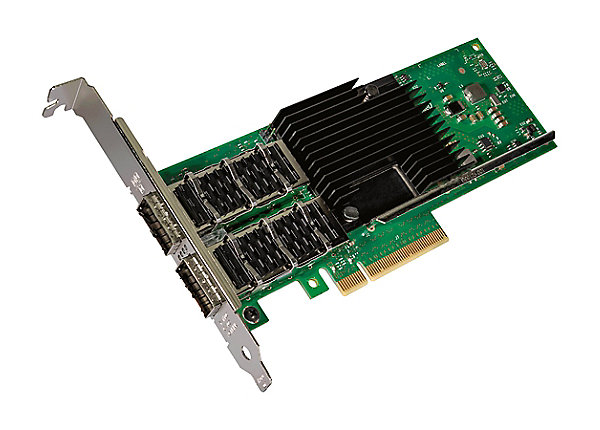
\includegraphics[width=0.60\textwidth]{pics/nic3}\\
\vspace{-1em}\tiny{Intel XL710 [Picture: Intel.com]}
\end{frame}

\begin{frame}{The ixy project}
\begin{itemize}
\item Attempt to write a simple yet fast user space network driver
\item It's a user space driver you can easily understand and read
\item $\approx$ 1,000 lines of C code, full of references to datasheets and specs
\item Supports Intel ixgbe NICs %(82599, X540, Xeon D, ...)
\item New: supports VirtIO NICs (qemu/kvm and VirtualBox, we got a Vagrant setup!)
\item Check it out on GitHub: \url{https://github.com/emmericp/ixy}
\end{itemize}
\end{frame}

\begin{frame}{Expectation: Beautiful C code}
\begin{itemize}
\item Why write a driver in C?
\pause
\vspace{1em}
\item Most drivers are written in C
\item C is the lowest common denominator of systems programming languages
\item C code can be beautiful
\item Everyone can read C?
\end{itemize}
\end{frame}

\begin{frame}[fragile]{Reality: C can be ugly}
\begin{minted}[autogobble]{c}
#define mystery_macro(ptr, type, member) ({\
	const typeof(((type*)0)->member)* __mptr = (ptr);\
	(type*)((char*)__mptr - offsetof(type, member));\
})
\end{minted}
\end{frame}

\begin{frame}[fragile]{Reality: C can be ugly}
\begin{minted}[autogobble]{c}
#define container_of(ptr, type, member) ({\
	const typeof(((type*)0)->member)* __mptr = (ptr);\
	(type*)((char*)__mptr - offsetof(type, member));\
})
\end{minted}
\end{frame}


\begin{frame}[fragile]{Reality: C can be ugly}
\begin{minted}[autogobble]{c}
#define container_of(ptr, type, member) ({\
	const typeof(((type*)0)->member)* __mptr = (ptr);\
	(type*)((char*)__mptr - offsetof(type, member));\
})
\end{minted}
\begin{itemize}
\item Allows some ``inheritance'' in C to abstract driver implementations
\item Virtually all C drivers use this macro
\item The Linux kernel contains $\approx$ 15,000 uses of this macro
\end{itemize}
\end{frame}

\begin{frame}{C can cause security problems}
\centering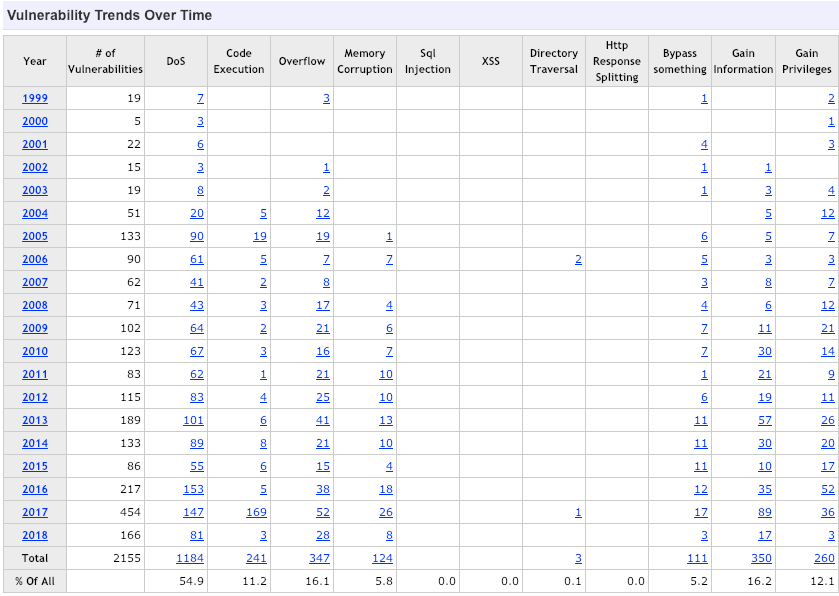
\includegraphics[trim={0 13cm 0 0},clip,width=0.65\textwidth]{pics/cve}

\footnotesize (...)

\centering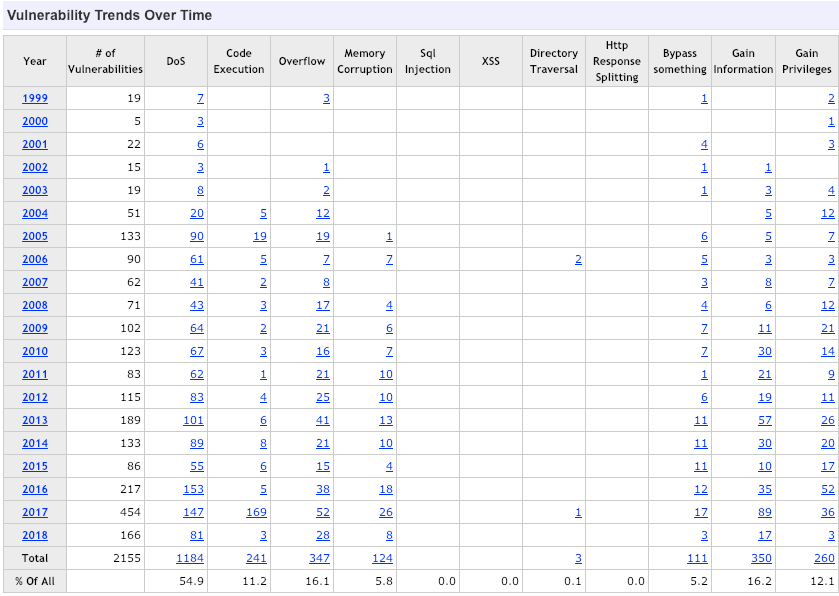
\includegraphics[trim={0 0 0 17.5cm},clip,width=0.65\textwidth]{pics/cve}

\begin{itemize}
\item Screenshot from \url{https://www.cvedetails.com/}
\item Security bugs found in the Linux kernel in the last $\approx$ 20 years
\end{itemize}

\end{frame}


\begin{frame}{C can cause security problems}
\begin{itemize}
\item Not all bugs can be blamed on the language
\item Cutler et al. analyzed 65 CVEs categorized as code execution in the Linux kernel \footnote{C. Cutler, M. F. Kaashoek, and R. T. Morris, \emph{``The benefits and costs of writing a POSIX kernel in a high-level language''}, USENIX OSDI, 2018}
\end{itemize}
\pause
\begin{table}
\centering
\begin{tabular}{ l  r r l }
  \toprule
  Bug type & Num. & Perc. & Can be avoided by language? \\
  \midrule
  Various & 11 & 17\% & Unclear/Maybe \\
  Logic & 14 & 22\% & No \\
  Use-after-free & 8 & 12\% & Yes \\
  Out of bounds & 32 & 49\% & Yes (likely leads to panic) \\
  \bottomrule  
\end{tabular}
\caption{Code execution vulnerabilities in the Linux kernel identified by Cutler et al$^1$}
\end{table}
\end{frame}

\begin{frame}{Are there preventable bugs in drivers?}
\begin{itemize}
\item We looked at these 40 preventable bugs
\pause
\item 39 of them were in drivers (the other was in the Bluetooth stack)
\pause
\item 13 were in the Qualcomm WiFi driver
\end{itemize}
\end{frame}

\begin{frame}{Should you really write new code in C in 2019?}
\begin{itemize}
\item If you have a choice: probably not, no
\pause
\item User space drivers can be written in \emph{any} language!
\item But are all languages an equally good choice?
\item Is a JIT compiler or a garbage collector a problem in a driver?
\end{itemize}
\end{frame}

\setbeamertemplate{footline}{}
\setbeamertemplate{headline}{}
\begin{frame}{}
\centering
\includegraphics[width=0.65\textwidth]{pics/allthe1}
\end{frame}

\begin{frame}{}
\centering
\includegraphics[width=0.65\textwidth]{pics/allthe2}
\end{frame}

\begin{frame}{}
\centering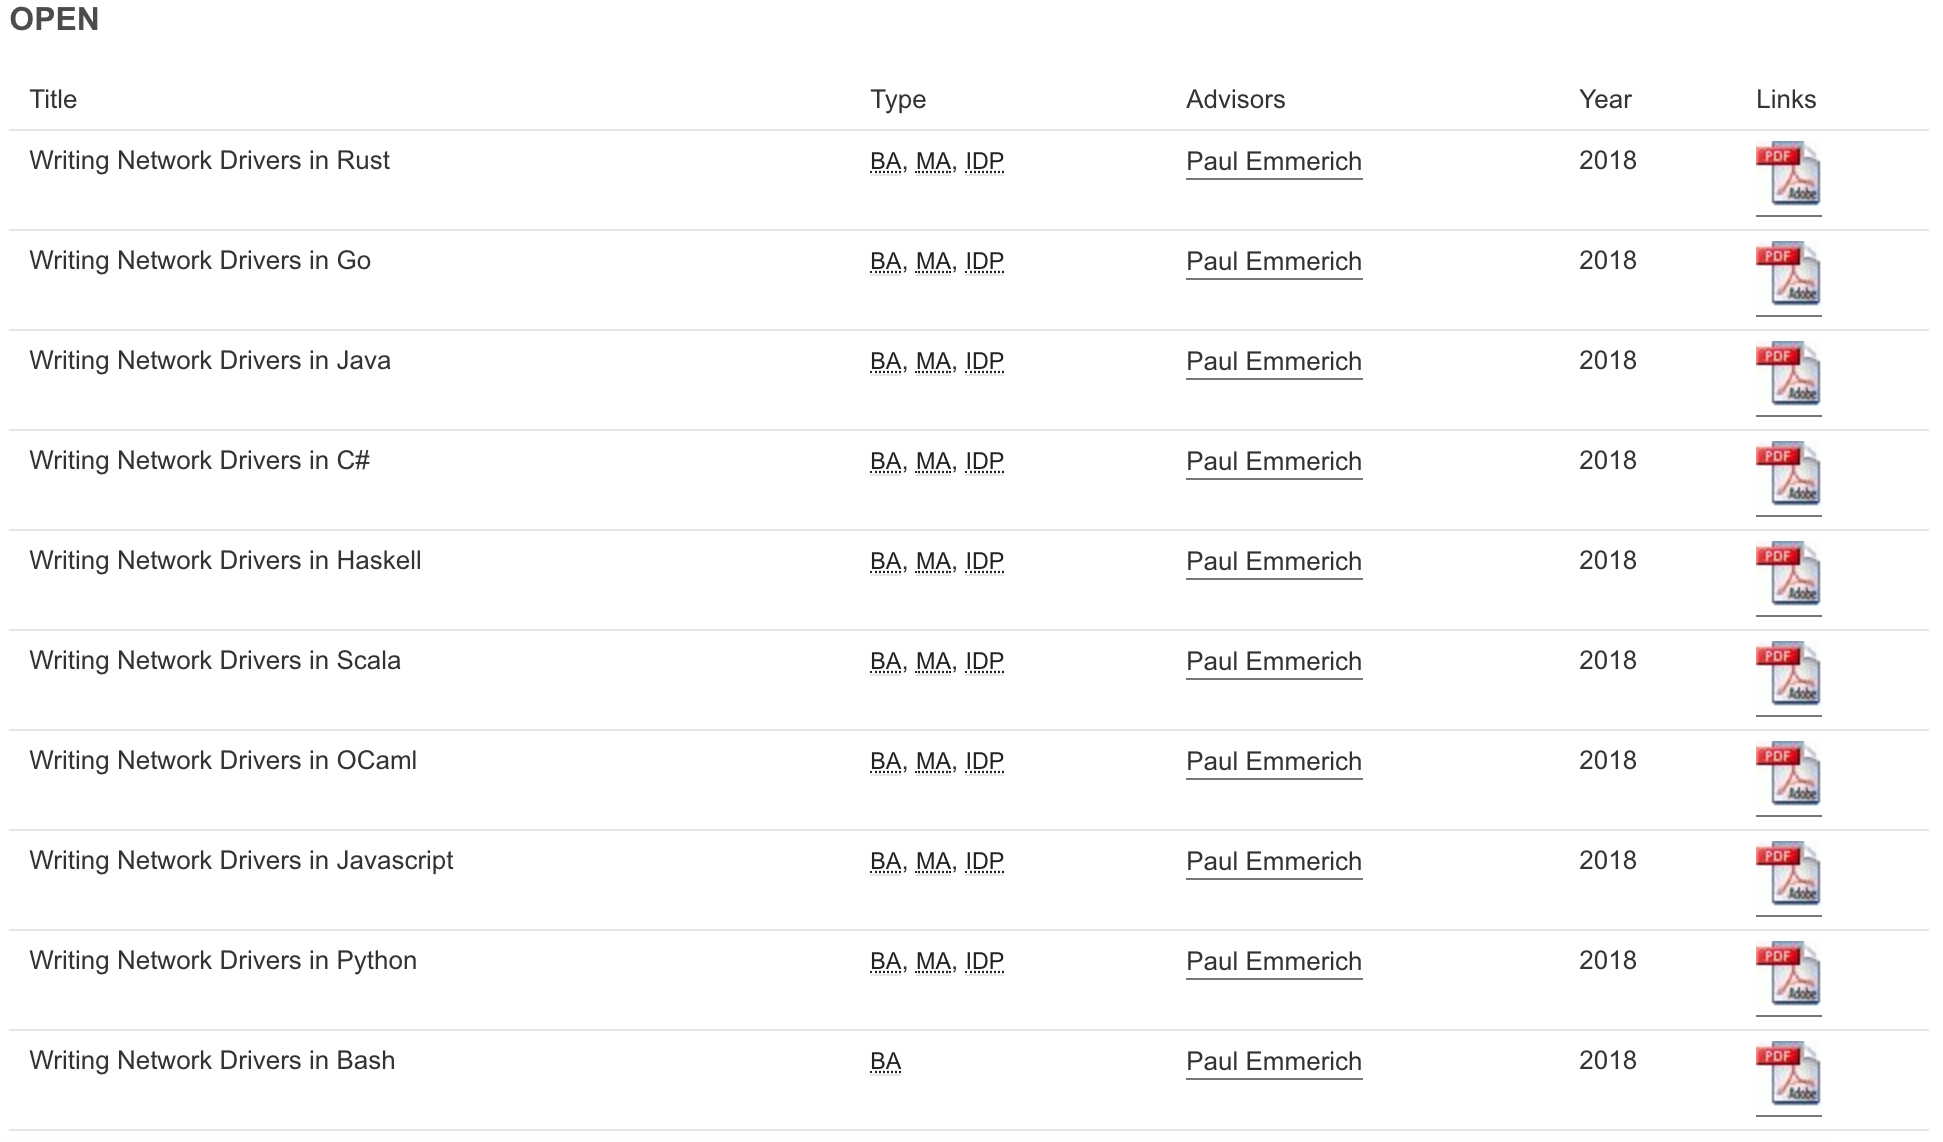
\includegraphics[width=0.85\textwidth]{pics/theses}
\end{frame}
\setbeamertemplate{headline}[tumheadline]
\setbeamertemplate{footline}[tumfootline]


\begin{frame}{Basics: How to talk to (modern) PCIe devices}
\begin{enumerate}
\item Memory-mapped IO (MMIO)
\item Direct memory access (DMA)
\item Interrupts
\end{enumerate}
\end{frame}

\begin{frame}{Basics: How to talk to (modern) PCIe devices}
\begin{enumerate}
\item Memory-mapped IO (MMIO)
\begin{itemize}
\item Magic memory area that is mapped to the device
\item Memory reads/writes are directly forwarded to the device
\item Usually used to expose device registers
\item User space drivers: \texttt{mmap} a magic file
\end{itemize}
\item[\color{TUMLightGray}2.] {\color{TUMLightGray} Direct memory access (DMA)}
\item[\color{TUMLightGray}3.] {\color{TUMLightGray} Interrupts}
\end{enumerate}
\end{frame}

\begin{frame}{Basics: How to talk to (modern) PCIe devices}
\begin{enumerate}
\item[\color{TUMLightGray}1.] {\color{TUMLightGray} Memory-mapped IO (MMIO)}
\item[2.] Direct memory access (DMA)
\begin{itemize}
\item Allows the device to read/write \emph{arbitrary} memory locations
\item User space drivers: figure out physical addresses, tell the device to write there
\end{itemize}
\item[\color{TUMLightGray}3.] {\color{TUMLightGray}  Interrupts}
\end{enumerate}
\end{frame}

\begin{frame}{Basics: How to talk to (modern) PCIe devices}
\begin{enumerate}
\item[\color{TUMLightGray}1.] {\color{TUMLightGray} Memory-mapped IO (MMIO)}
\item[\color{TUMLightGray}2.] {\color{TUMLightGray} Direct memory access (DMA)}
\item[3.] Interrupts
\begin{itemize}
\item This is how the device informs you about events
\item User space drivers: available via the Linux \texttt{vfio} subsystem
\item (Usually) not useful for high-speed network drivers 
\item We'll ignore interrupts here
\end{itemize}
\end{enumerate}
\end{frame}


\begin{frame}{Basics: How to write a user space driver in 4 simple steps}
\begin{itemize}
\item[1.] Unload kernel driver
\item[2.] \texttt{mmap} the PCIe MMIO address space
\item[3.] Figure out physical addresses for DMA
\item[4.] Write the driver
\end{itemize}
\end{frame}

\begin{frame}{Hardware: Intel \texttt{ixgbe} family (10\,Gbit/s)}
\begin{itemize}
\item \texttt{ixgbe} family: 82599ES (aka X520), X540, X550, Xeon D embedded NIC
\item Commonly found in servers or as on-board chips
\item Very good datasheet publicly available
\vspace{1em}
\item Almost no logic hidden behind black-box firmware
%\item<2-> Black-box firmware contains almost no magic
\item<2-> Drivers for many newer NICs often just exchanges messages with the firmware
\item<2-> Here: all hardware features directly exposed to the driver
\end{itemize}
\end{frame}



\newmintinline[ccode]{c}{}
\newmintinline[bashcode]{c}{}

\begin{frame}[fragile=singleslide]{Find the device we want to use}
\begin{Verbatim}[commandchars=\\\{\}]
# lspci
03:00.0 Ethernet controller: Intel Corporation 82599ES 10-Gigabit SFI/SFP+ ...
03:00.1 Ethernet controller: Intel Corporation 82599ES 10-Gigabit SFI/SFP+ ...
\end{Verbatim}
\end{frame}

\begin{frame}[fragile=singleslide]{Find the device we want to use}
\begin{Verbatim}[commandchars=\\\{\}]
# lspci
\textbf{03:00.0} Ethernet controller: Intel Corporation 82599ES 10-Gigabit SFI/SFP+ ...
\textbf{03:00.1} Ethernet controller: Intel Corporation 82599ES 10-Gigabit SFI/SFP+ ...
\end{Verbatim}
\end{frame}

\begin{frame}[fragile=singleslide]{Unload the kernel driver}
\begin{minted}{bash}
echo 0000:03:00.1 > /sys/bus/pci/devices/0000:03:00.1/driver/unbind
\end{minted}
\end{frame}

\begin{frame}[fragile=singleslide]{\texttt{mmap} the PCIe configuration address space from user space}
\begin{minted}[autogobble]{c}
int fd = open("/sys/bus/pci/devices/0000:03:00.0/resource0", O_RDWR);
struct stat stat;
fstat(fd, &stat);
uint8_t* registers = (uint8_t*) mmap(NULL, stat.st_size, PROT_READ | PROT_WRITE,
                                     MAP_SHARED, fd, 0);
\end{minted}
\end{frame}

\begin{frame}{Device registers}
\centering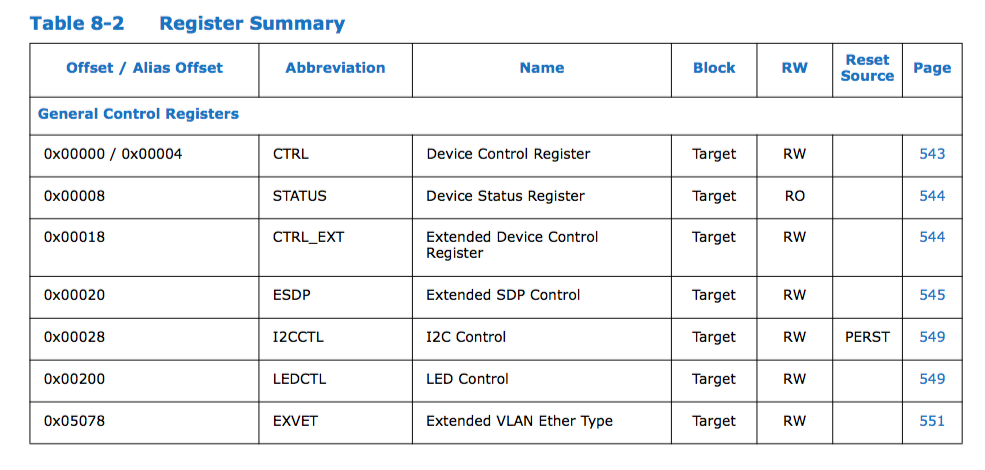
\includegraphics[width=0.75\textwidth]{pics/registers}
\end{frame}

\begin{frame}[fragile=singleslide]{Access registers: LEDs}
\begin{minted}[autogobble]{c}
#define LEDCTL 0x00200
#define LED0_BLINK_OFFS 7

uint32_t leds = *((volatile uint32_t*)(registers + LEDCTL));
*((volatile uint32_t*)(registers + LEDCTL)) = leds | (1 << LED0_BLINK_OFFS);
\end{minted}
\begin{itemize}
\item Memory-mapped IO: all memory accesses go directly to the NIC
\item One of the very few valid uses of \ccode{volatile} in C
\end{itemize}
\end{frame}


\begin{frame}{Handling packets via DMA}
\begin{itemize}
\item Packets are transferred via queue interfaces (often called rings)
\item Rings are configured via MMIO and accessed via by the device DMA
\item Rings (usually) contain pointers to packets, also accessed via DMA
\pause
\vspace{1em}
\item Details vary between different devices
\item This is not unique to NICs: most PCIe devices work in a similar manner
\end{itemize}
\end{frame}


\begin{frame}{Challenges for high-level languages}
\begin{itemize}
\item Access to \texttt{mmap} with the proper flags
\item Handle externally allocated (foreign) memory in the language
\item Handle memory layouts/formats (i.e., access memory that looks like a given C struct)
\item Memory access semantics: memory barriers, volatile reads/writes
\item Some operations in drivers are inherently unsafe
\end{itemize}
\end{frame}


\begin{frame}{Goals for our implementations}
\begin{itemize}
\item Implement the same feature set as my C reference driver
\item Use a similar structure like the C driver
\item Write idiomatic code for the selected language
\item Use language safety features where possible
\item Quantify trade-offs for performance vs. safety
\end{itemize}
\end{frame}

\setbeamertemplate{footline}{}
\setbeamertemplate{headline}{}
\setbeamertemplate{headline}[tumheadline]
\setbeamertemplate{footline}[tumfootline]
\begin{frame}{}
\centering \scalebox{4}{\Huge C\#}
\end{frame}


\begin{frame}{C\#}
\begin{itemize}
\item No, we didn't develop a Windows driver
\item We used Microsoft's CoreCLR on Linux
\pause
\vspace{1em}
\item JIT compiled
\item Garbage collected
\item Memory safe (mostly)
\pause
\vspace{1em}
\item C\# supports a relatively obscure \emph{unsafe mode}
\item Unsafe mode features full support for pointers
\end{itemize}
\end{frame}

\begin{frame}[fragile]{C\#: Access to external memory}
\begin{itemize}
\item C\# provides \texttt{UnmanagedMemoryStream}, a nice wrapper for foreign memory
\item But it was too slow :(
\pause
\item Use unsafe raw pointers for packet buffers instead
\end{itemize}
\begin{minted}[autogobble]{csharp}
public unsafe void WriteData(uint offset, int val) {
    if (offset >= BUF_SIZE) throw new IndexOutOfRangeException();
    int *ptr = (int*)(_baseAddress + DataOffset + offset);
    *ptr = val;
}
\end{minted}
\begin{itemize}
\pause
\item Looks a lot like C
\item Potentially unsafe operations are all in a few known places, simpler auditing
\end{itemize}
\end{frame}


%\begin{frame}[]{C\#: Summary}
%\begin{itemize}
%\item ???
%\end{itemize}
%\end{frame}

\setbeamertemplate{footline}{}
\setbeamertemplate{headline}{}
\begin{frame}{}
\centering
\includegraphics[width=0.8\textwidth]{pics/swift}
\end{frame}
\setbeamertemplate{headline}[tumheadline]
\setbeamertemplate{footline}[tumfootline]

\begin{frame}{Swift}
\begin{itemize}
\item No, we didn't develop a macOS/iOS driver
\item Swift is also available on Linux
\pause
\vspace{1em}
\item Compiled via LLVM
\item Memory management via reference counting (ARC)
\item Memory safe (mostly)
%\pause
%\vspace{1em}
%\item Access to external memory via \texttt{UnsafeBufferPointer} 
\end{itemize}
\end{frame}

\begin{frame}[fragile]{Swift: Pointers}
\begin{itemize}
\item \texttt{UnsafeBufferPointer} and co wrap foreign memory blobs
\item Used to make packets in DMA buffers available
\end{itemize}
\begin{minted}[autogobble]{swift}
public var packetData: UnsafeBufferPointer<UInt8>? {
    get {
        return UnsafeBufferPointer<UInt8>(
            start: self.entry.pointer.assumingMemoryBound(to: UInt8.self),
            count: Int(self.size)
        )
    }
}
\end{minted}
\begin{itemize}
\item Forces you to specify the buffer size, accesses check the bounds in debug mode
\end{itemize}
\end{frame}

\begin{frame}[fragile]{Swift: Pointers with a very verbose syntax}
\begin{itemize}
\item Example: modify one byte in a packet (part of our benchmark)
\end{itemize}
\begin{minted}[autogobble]{swift}
public func touch() {
    let ptr = self.entry.pointer
    var newValue: UInt32 = ptr.load(fromByteOffset: 0, as: UInt32.self)
    newValue += 1
    ptr.storeBytes(of: newValue, toByteOffset: 0, as: UInt32.self)
}
\end{minted}
\begin{itemize}
\item Quite verbose compared to C or C\#
\end{itemize}
\end{frame}



\setbeamertemplate{footline}{}
\setbeamertemplate{headline}{}
\begin{frame}{}
\centering
\includegraphics[width=0.8\textwidth]{pics/ocaml}
\end{frame}
\setbeamertemplate{headline}[tumheadline]
\setbeamertemplate{footline}[tumfootline]

\begin{frame}{OCaml}
\begin{itemize}
\item Compiled language
\item Memory management via garbage collection
\item Memory safe
\item Functional language
\end{itemize}
\end{frame}


\begin{frame}[fragile]{OCaml: Cstruct}
\begin{minted}[autogobble]{ocaml}
[%%cstruct
  type adv_rxd_wb = {
    pkt_info : uint16;
    hdr_info : uint16;
    ip_id : uint16;
    csum : uint16;
    status_error : uint32;
    length : uint16;
    vlan : uint16
  } [@@little_endian]
]
\end{minted}
\begin{itemize}
\item Cstruct generates accessors to work with (foreign) memory that looks like this
\end{itemize}
\end{frame}

\begin{frame}[fragile]{OCaml: It looks quite different}
\begin{itemize}
\item Code that checks how many packets are ready to be read in the receive ring
\end{itemize}
\begin{minted}[autogobble]{ocaml}
let num_done =
  let rec loop offset =
    let rxd = descriptors.(wrap_rx (rxq.rx_index + offset)) in
    if Int32.((get_adv_rx_wb_status rxd) land RXD.stat_dd <> 0l) then
      loop (offset + 1)
    else
      offset in
  loop 0
\end{minted}
\end{frame}


%\begin{frame}[fragile]{OCaml: It looks quite different}
%\begin{itemize}
%\item Example of the forwarder application on top of the driver
%\end{itemize}
%\begin{minted}[autogobble]{ocaml}
%let forward rx_dev tx_dev =
%  let rx = Ixy.rx_batch rx_dev 0 in
%  Ixy.tx_batch_busy_wait tx_dev 0 rx
%\end{minted}
%\end{frame}


\setbeamertemplate{footline}{}
\setbeamertemplate{headline}{}
\begin{frame}{}
\centering
\includegraphics[width=0.6\textwidth]{pics/haskell}
\end{frame}
\setbeamertemplate{headline}[tumheadline]
\setbeamertemplate{footline}[tumfootline]

\begin{frame}{Haskell}
\begin{itemize}
\item Compiled language (GHC)
\item Memory management via garbage collection
\item Memory safe
\item Functional language
\end{itemize}
\end{frame}


\begin{frame}{Haskell: Access to foreign memory}
\begin{itemize}
\item \texttt{mmap} and \texttt{mlock} available via \texttt{System.Posix.Memory}
\begin{itemize}
\item All necessary flags and features are available in Haskell, we had to write some C code to get \texttt{mmap/mlock} in OCaml
\end{itemize}
\vspace{1em}
\item \texttt{Foreign} package provides access to foreign memory
\end{itemize}
\end{frame}


\begin{frame}[fragile]{Haskell: Sum types are useful}
\begin{itemize}
\item Descriptors often exist in two forms
\begin{itemize}
\item One format written by the driver and read by the device
\item A second format that is written back by the device once it's finished
\end{itemize}
\end{itemize}
\begin{minted}{haskell}
data TransmitDescriptor = TransmitRead { tdBufPhysAddr :: !Word64
                                       , tdCmdTypeLen :: !Word32
                                       , tdOlInfoStatus :: !Word32 }
                          | TransmitWriteback { tdStatus :: !Word32 }
\end{minted}
\end{frame}


\begin{frame}[fragile]{Haskell: How to write a TX descriptor}
\begin{minted}{haskell}
unsafeUseAsCStringLen pkt (\(ptr, len) -> copyBytes bufPtr (castPtr ptr) len)
poke descPtr TransmitRead { tdBufPhysAddr = bufPhysAddr 
                          , tdCmdTypeLen = fromIntegral $ cmdTypeLen size
                          , tdOlInfoStatus = fromIntegral $ shift size 14 }
writeIORef (txqIndexRef queue) nextIndex
\end{minted}
\end{frame}




\setbeamertemplate{footline}{}
\setbeamertemplate{headline}{}
\begin{frame}{}
\centering
\includegraphics[width=0.8\textwidth]{pics/go}
\end{frame}
\setbeamertemplate{headline}[tumheadline]
\setbeamertemplate{footline}[tumfootline]

\begin{frame}{Go}
\begin{itemize}
\item Compiled programming language developed by Google 
\item General purpose language but designed for distributed systems
\item<2-> A driver is not a distributed system
\item<3-> Then why even use Go?
\begin{itemize}
\item<4-> Runtime for:\\Garbage Collection\\Memory \& Type safety
%\item<4-> Simple yet powerful concurrency via goroutines	%not relevant ofr a single core driver
\item<4-> Large standard library
\end{itemize}
\end{itemize}
\end{frame}

\begin{frame}{Go for Drivers}
\begin{itemize}
\item Actually a lot like C in many aspects
%maybe include some code examples?
\item<2-> Main differences:
\begin{itemize}
\item<2-> No pointer arithmetic (managing DMA memory)
\item<2-> No volatile (memory barriers for register access)
\end{itemize}
\item<3-> What we do instead:
\begin{itemize}
\item<3-> Manage DMA memory via slices
\item<3-> Unsafe pointers: circumvent runtime but allow arbitrary pointer\\
	$\rightarrow$ Physical address calculation \& register access
\item<3-> Rule set for unsafe pointers to still be valid
\end{itemize}
\end{itemize}
\end{frame}

\begin{frame}[fragile]{Managing Memory: Mempools}
\begin{itemize}
\item syscall.Mmap() returns slice of the mmapped memory area
\item For this presentation: slice = fancy array\\
	$\rightarrow$ bounds checked, subslicing, etc.
\end{itemize}
%\end{frame}

%\begin{frame}[fragile]{func MemoryAllocateMempool}
%mempool alloc code
\begin{minted}[autogobble]{go}
//allocate DMA memory & initialize mempool
for i := uint32(0); i < numEntries; i++ {
	mempool.packetBuf[i] = &PktBuf{
		Pkt:        mempool.buf[i*entrySize : (i+1)*entrySize],
		PhyAddr:    uint64(virtToPhys(uintptr(
			    unsafe.Pointer(&mempool.buf[i*entrySize])))),
	}
}
\end{minted}
\end{frame}

\begin{frame}[fragile]{No volatile no problem}
%insert code registers
\begin{itemize}
\item Registers share memory with NIC
\item Memory barrier to prevent re-ordering
\item sync/atomic functions prevent re-ordering around them
\end{itemize}
\begin{minted}[autogobble]{go}
func setReg32(addr []byte, reg int, value uint32) {
	atomic.StoreUint32((*uint32)(unsafe.Pointer(&addr[reg])), value)
}

func getReg32(addr []byte, reg int) uint32 {
	return atomic.LoadUint32((*uint32)(unsafe.Pointer(&addr[reg])))
}
\end{minted}
\end{frame}

\begin{frame}{Conclusion Go}
\begin{itemize}
\item Actually quite nice to work with
\begin{itemize}
\item Safety (see Cutler et al.\footnote{C. Cutler, M. F. Kaashoek, and R. T. Morris, \emph{``The benefits and costs of writing a POSIX kernel in a high-level language''}, USENIX OSDI, 2018})
\item Looks like C in beautiful
\end{itemize}
\item<2-> But
\begin{itemize}
\item<2-> Approx 10\% slower then C % at optimum batch size
%\item<2-> Needs higher batch sizes to be efficient
\item<2-> Descriptor access can be ugly (functions on descriptors are too costly)
\end{itemize}
\end{itemize}
\end{frame}

\setbeamertemplate{footline}{}
\setbeamertemplate{headline}{}
\begin{frame}{}
\centering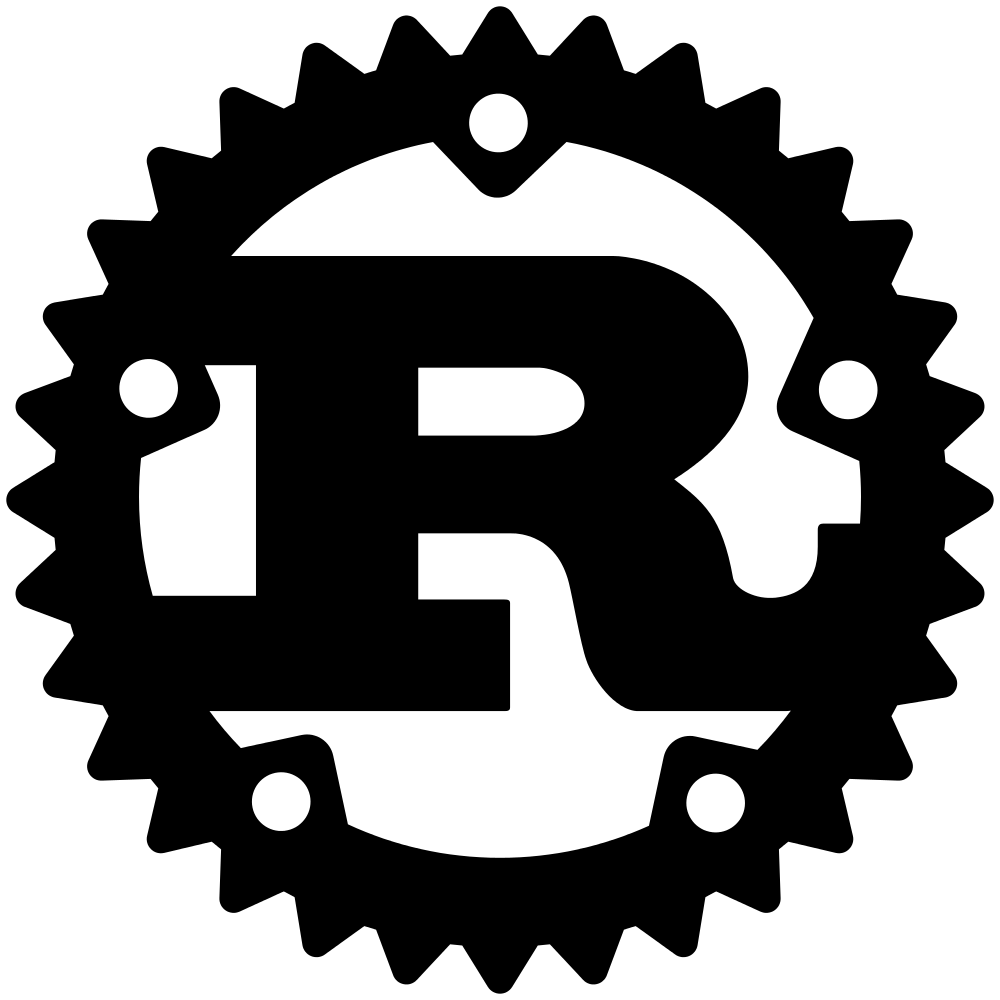
\includegraphics[height=0.87\textheight]{pics/rust}
\end{frame}
\setbeamertemplate{headline}[tumheadline]
\setbeamertemplate{footline}[tumfootline]

\begin{frame}{Rust}
\emph{What is Rust?}\\
\begin{quote}
A safe, concurrent, practical systems language.
\end{quote}\\
Great! That's what we are looking for! Anything else we need to know?\\
\begin{itemize}
\item No garbage collector
\item Unique ownership system and rules for moving/borrowing values
\item Unsafe mode
\end{itemize}
\end{frame}

\begin{frame}{Safety in Rust: The Ownership System}
\begin{itemize}
%\item Immutability of variables by default
\item Three rules:
\begin{enumerate}
\item Each value has a variable that is its owner
\item There can only be one owner at a time
\item When the owner goes out of scope, the value is freed
\end{enumerate}
\item Rules enforced at compile-time
\item Ownership can be passed to another variable% by
%\begin{itemize}
%\item ``moving'' the value or by
%\item ``borrowing'' it through a reference
%\end{itemize}
\end{itemize}
\end{frame}

\begin{frame}[fragile]{Safety in Rust: The Ownership System by Example}
\begin{itemize}
\item \texttt{Packet}s are owners of some DMA memory
\item \texttt{Packet}s are passed between users and the driver, thus ownership is passed as well
\item At any point in time there is only one \texttt{Packet} owner that can change its memory
\end{itemize}
\begin{minted}{rust}
let buffer: &mut VecDeque<Packet> = VecDeque::new();
dev.rx_batch(RX_QUEUE, buffer, BATCH_SIZE);
for p in buffer.iter_mut() {
  p[48] += 1;
}
dev.tx_batch(TX_QUEUE, buffer);
buffer.drain(..);
\end{minted}
\end{frame}

\begin{frame}[fragile]{Safety in Rust: Unsafe Code}
\begin{itemize}
\item Not everything can be done in safe Rust
\item Calling foreign functions and dereferencing raw pointers is per se unsafe
\item Many functions in Rust's standard library make use of unsafe code
\end{itemize}
\begin{minted}{rust}
let ptr = unsafe {
  libc::mmap(
    ptr::null_mut(), len, libc::PROT_READ | libc::PROT_WRITE,
    libc::MAP_SHARED, file.as_raw_fd(), 0,
  ) as *mut u8
};
\end{minted}
\end{frame}

\begin{frame}[fragile]{Rust by Example}
\begin{itemize}
\item Biggest challenge: safe memory handling with unsafe code
\end{itemize}
\begin{minted}{rust}
fn set_reg32(&self, reg: u32, val: u32) {
  assert!(
    reg as usize <= self.len - 4 as usize,
    "memory access out of bounds"
  );

  unsafe {
    ptr::write_volatile((self.addr as usize + reg as usize) as *mut u32, val);
  }
}
\end{minted}
\end{frame}

\begin{frame}{Performance comparison}
\centering\includestandalone[scale=0.8]{figures/benchmarks-all-throughput}
\end{frame}

\begin{frame}{Batching at 1.6,\GHz CPU speed}
\centering\includestandalone[scale=0.8]{figures/benchmarks-all-batching}
\end{frame}

\setbeamertemplate{footline}{}
\setbeamertemplate{headline}{}
\begin{frame}{Swift: Flame graph}
\hspace{-.5cm}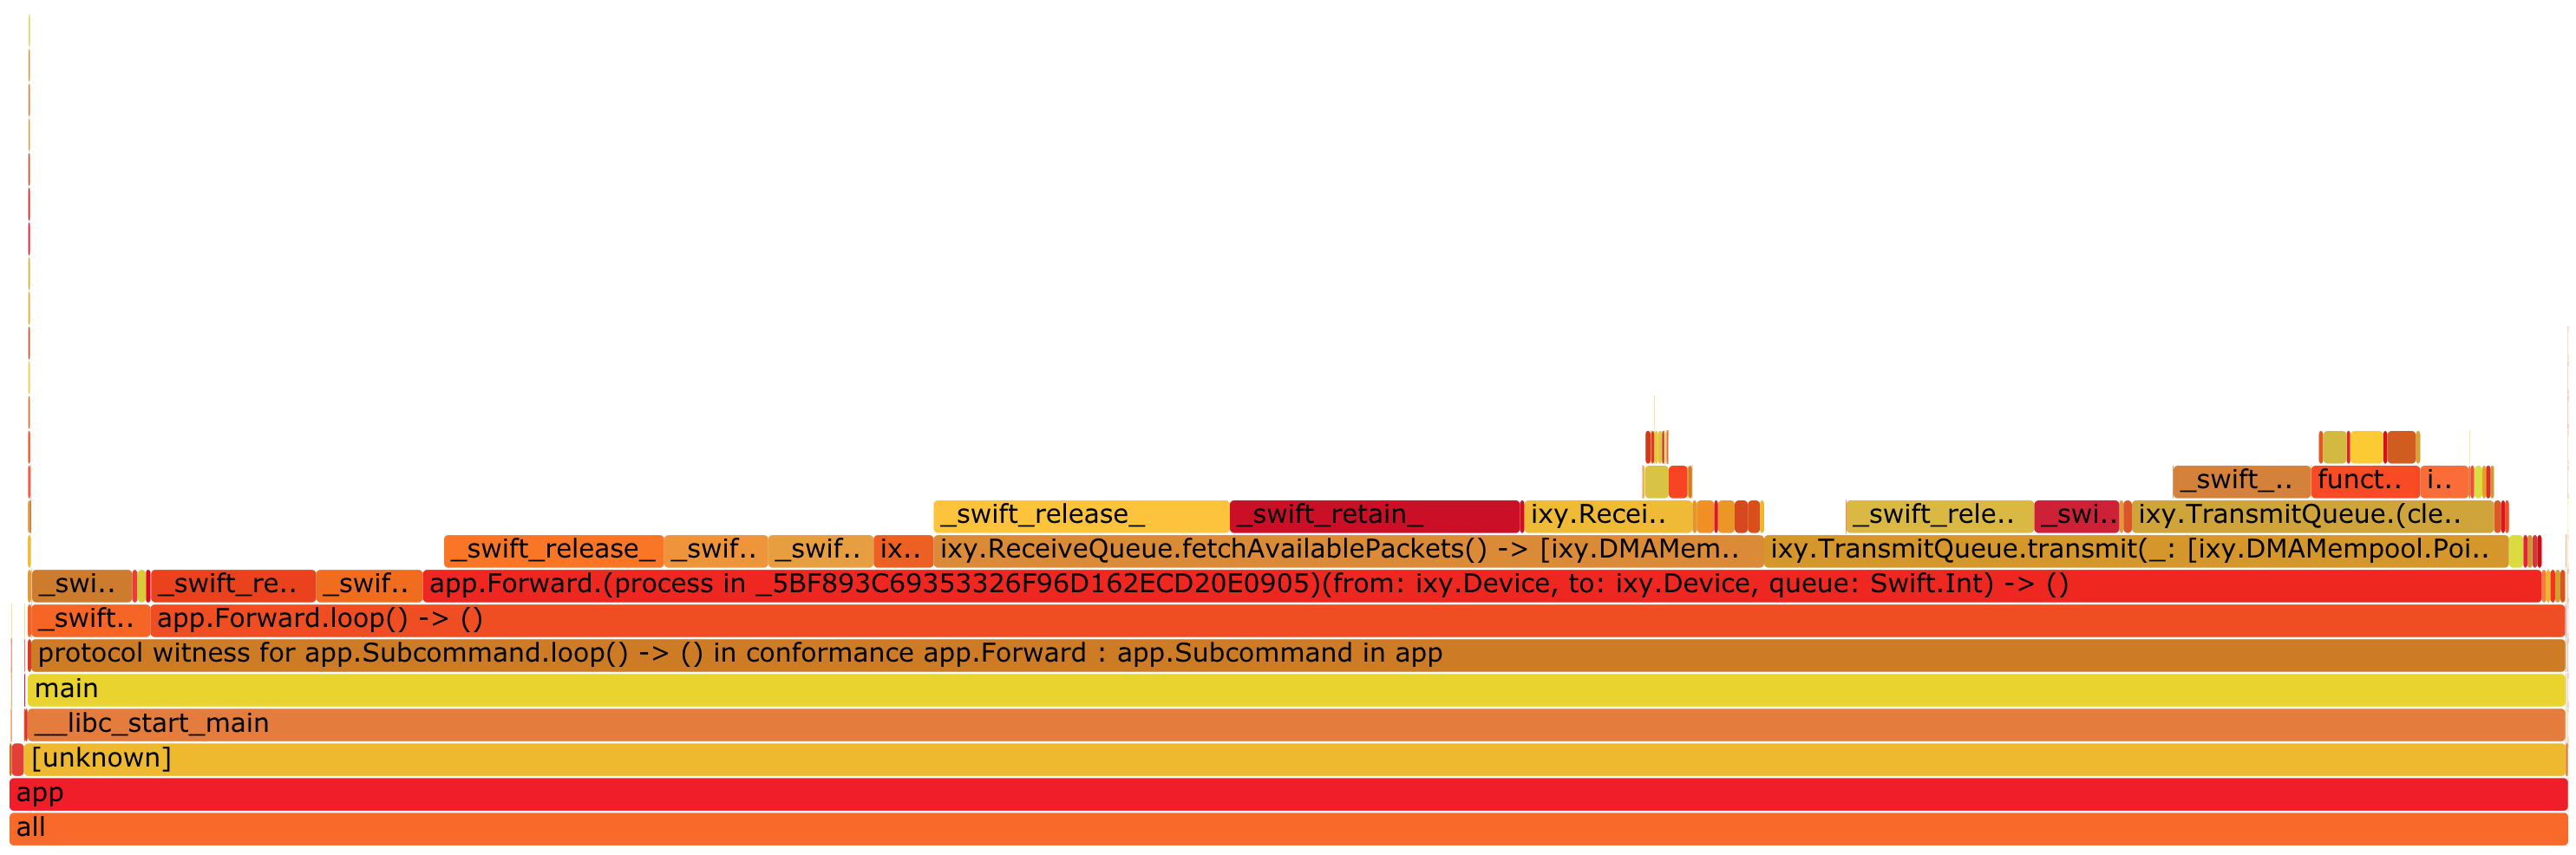
\includegraphics[width=1.065\textwidth]{pics/flamegraph}
\end{frame}
\setbeamertemplate{footline}[tumfootline]
\setbeamertemplate{headline}[tumheadline]

\begin{frame}{Swift: Why so slow?}
\begin{itemize}
\item Lots of time spent in Swift's memory management
\item Swift adds calls to release/retain for each used object in each function
\item This is basically the same as wrapping every object in a \texttt{std::shared\_ptr} in C++
\vspace{1em}
\pause
\item Time in release/retain: 76\%
\item For comparison: Go spends less than 0.5\% in the garbage collector
\end{itemize}
\end{frame}

\begin{frame}{Garbage collection and JIT compilation vs. latency}
\centering\includestandalone[scale=0.8]{figures/latency-cdf1}
\end{frame}

\begin{frame}{Garbage collection and JIT compilation vs. latency}
\centering\includestandalone[scale=0.8]{figures/latency-cdf2}
\end{frame}

\begin{frame}{Garbage collection and JIT compilation vs. latency}
\centering\includestandalone[scale=0.8]{figures/latency-cdf3}
\end{frame}

\begin{frame}{Garbage collection and JIT compilation vs. latency}
\centering\includestandalone[scale=0.8]{figures/latency-cdf4}
\end{frame}

\begin{frame}{Complementary cumulative distribution function}
\centering\includestandalone[scale=0.8]{figures/latency-ccdf}
\end{frame}

\begin{frame}{Tail latency}
\centering\includestandalone[scale=0.8]{figures/latency-hdr-hist}
\end{frame}


\begin{frame}{Look ma, no root}
\begin{itemize}
\item User space drivers usually run with root privileges, but why?
\pause
\vspace{1em}
\item Mapping PCIe resources requires root
\item Allocating non-transparent huge pages requires root
\item Locking memory requires root
\vspace{1em}
\item Can we do that in a small separate program that is easy to audit and then drop privileges?
\pause
\item Yes, we can
\item But it's not really secure
\end{itemize}
\end{frame}

\begin{frame}{Memory access on modern systems}
\centering\includestandalone[scale=.75]{figures/iommu1}
\end{frame}

\begin{frame}{Unprivileged user space drivers on Linux}
\begin{itemize}
\item[1.] Prepare the system as root
\begin{itemize}
\item[1.1.] Bind the device to the special \texttt{vfio} driver
\item[1.2.] \texttt{chown} the special magic \texttt{vfio} device to your user
\item[1.3.] Allow your user to lock some amount of memory via \texttt{ulimit}
\end{itemize}
\pause
\item[2.] \texttt{mmap} the special magic \texttt{vfio} device
\item[3.] Do some magic \texttt{ioctl} calls on the magic device
\item[4.] Protected DMA memory can also be allocated via an \texttt{ioctl} call
\item[5.] Use the device as usual, all accesses are now checked by the IOMMU
\vspace{1em}
\pause
\item We have implemented this in our C driver, Rust is WIP
\end{itemize}
\end{frame}




\begin{frame}{Why write a user space network driver?}
\begin{itemize}
\item Why not? It can be fun
\item Maybe you need a quick \& dirty driver for a weird device?
\item Maybe you need quick development cycles while playing around with a custom device
\item Maybe you need some feature not supported by the original driver
\end{itemize}
\end{frame}


\begin{frame}{Example: Hardware timestamping}
\begin{itemize}
\item Our latency measurement requires timestamps with nanosecond-level precision
\item It also needs to handle millions of packets per second (we measured with $\approx$ 15\,Mpps)
\item This usually requires special hardware (we've used NetFPGAs to do this in the past)
\pause
\vspace{1em}
\item Some cheap off-the-shelf NICs can add a timestamp to all  incoming packets
\item But none of the existing drivers support this feature :(
\pause
\item We just set some flags in the right registers and got precise timestamping for cheap
\item We used a Xeon D embedded NIC capturing all packets via a fiber optic splitter before and after our device under test (precision $\approx$ \textpm 15\,ns)
\end{itemize}
\end{frame}

%\begin{frame}{(Maybe) network stack of the future}
%\end{frame}

\begin{frame}{Conclusion: Check out our code}
%\centering \qrcode[height=3cm]{https://github.com/ixy-languages/ixy-languages}
\begin{itemize}
\item Meta-repository with links: \url{https://github.com/ixy-languages/ixy-languages}
\item Drivers are simple: don't be afraid of them
\item No kernel code needed :)
\end{itemize}
%\centering \Huge Q \& A
\end{frame}





\end{document}

